\documentclass[twocolumn,10pt]{article}
\usepackage[margin=1in]{geometry}
\usepackage{graphicx}
\usepackage{float}
\usepackage{booktabs}
\usepackage{microtype}
\usepackage{url}
\usepackage{amsmath}
\usepackage[hidelinks]{hyperref}
\usepackage{fancyhdr}

% Easter-egg citations: every reference title and every bracketed citation
% is an unstyled (hidelinks) external hyperlink to the cited paper. Each
% bibkey's URL is declared ONCE here; \ecite and \reftitle look it up, so a
% source URL is changed in exactly one place.
%   \paperurl{key}{url}      declare the URL for a bibkey
%   \ecite{key}               cite, linked externally (\NoHyper suppresses
%                             hyperref's internal bibliography link)
%   \reftitle{key}{Title}    linked title for use inside \bibitem
\newcommand{\paperurl}[2]{\expandafter\def\csname paperurl@#1\endcsname{#2}}
\newcommand{\paperurlof}[1]{\csname paperurl@#1\endcsname}
\newcommand{\ecite}[1]{\href{\paperurlof{#1}}{\NoHyper\cite{#1}\endNoHyper}}
\newcommand{\reftitle}[2]{\href{\paperurlof{#1}}{#2}}

\paperurl{lightsociety}{https://arxiv.org/abs/2506.12078}
\paperurl{matraix}{https://arxiv.org/abs/2608.04205}
\paperurl{park2023}{https://arxiv.org/abs/2304.03442}
\paperurl{sentiment140}{https://www-cs.stanford.edu/people/alecmgo/papers/TwitterDistantSupervision09.pdf}
\paperurl{tweeteval}{https://aclanthology.org/2020.findings-emnlp.148/}
\paperurl{kwak2010}{https://snap.stanford.edu/class/cs224w-readings/kwak10twitter.pdf}
\paperurl{horton1956}{https://www.participations.org/03-01-04-horton.pdf}
\paperurl{degroot1974}{https://doi.org/10.1080/01621459.1974.10480137}
\paperurl{oasis}{https://arxiv.org/abs/2411.11581}
\paperurl{agentsociety}{https://arxiv.org/abs/2502.08691}
\paperurl{ysocial}{https://arxiv.org/abs/2408.00818}
\paperurl{socioverse}{https://arxiv.org/abs/2504.10157}
\paperurl{aps}{https://arxiv.org/abs/2605.27419}
\paperurl{poorman}{https://arxiv.org/abs/2608.11215}
\paperurl{hybriddiffusion}{https://arxiv.org/abs/2510.16366}
\paperurl{toposim}{https://arxiv.org/abs/2604.18011}
\paperurl{scaling}{https://arxiv.org/abs/2607.02464}
\paperurl{park2024}{https://arxiv.org/abs/2411.10109}
\paperurl{twin2k}{https://arxiv.org/abs/2505.17479}
\paperurl{blueprint}{https://arxiv.org/abs/2510.02343}
\paperurl{behaviorchain}{https://arxiv.org/abs/2502.14642}
\paperurl{personaarena}{https://arxiv.org/abs/2605.17044}
\paperurl{boundary}{https://arxiv.org/abs/2506.19806}
\paperurl{kramer2014}{https://doi.org/10.1073/pnas.1320040111}
\paperurl{ferrara2015}{https://arxiv.org/abs/1506.06021}
\paperurl{charlton2016}{https://arxiv.org/abs/1604.03427}
\paperurl{aral2009}{https://doi.org/10.1073/pnas.0908800106}
\paperurl{shalizi2011}{https://arxiv.org/abs/1004.4704}
\paperurl{tan2011}{https://arxiv.org/abs/1109.6018}
\paperurl{friedkin1990}{https://escholarship.org/uc/item/2r82w1vs}
\paperurl{huberman2009}{https://firstmonday.org/ojs/index.php/fm/article/view/2317}
\paperurl{cha2010}{https://ojs.aaai.org/index.php/ICWSM/article/view/14033}
\paperurl{golder2011}{https://doi.org/10.1126/science.1202775}
\pagestyle{plain}

\title{\textbf{popsim}: Reproducing Elements of Billion-Agent Social Simulators\\
on a Single Machine, with a Behavioral-Adherence Benchmark\\
for Persona Agents on Sentiment140}
\author{
  Micah Stubbs\\
  \texttt{micah@casemirror.ai}
  \and
  Yvonne Chen\\
  \texttt{yc.yvonnechen@gmail.com}
}
\date{August 2026}

\begin{document}
\maketitle

\begin{abstract}
Population-scale social simulators such as Light Society (one billion agents)
and MatrAIx (8.3 billion personas) require infrastructure most researchers
cannot access. We show that their core methodology of human-grounded personas,
tiered compute, and ground-truth validation runs on one commodity machine,
using Sentiment140: 1.6M public tweets in under 300\,MB of memory. We mine
personas for the 6{,}245 users with at least 20 tweets each, and a
mixture-of-models ladder cuts simulation cost $702.7\times$ versus an all-LLM
population. Validating on the real @-mention graph produces a negative result:
DeGroot opinion diffusion ($r=0.54$) underperforms per-user persistence
($r=0.73$) at predicting future sentiment. Disposition beats diffusion.
Sustained one-way (parasocial) attachments prove as numerous as strong mutual
ties, motivating a near-zero-cost broadcast tier. We also release a fixed
behavioral-adherence benchmark: per-user temporal 80/20 splits scored on
42{,}998 held-out tweets, where a zero-parameter persona baseline reaches
63.1\% and MatrAIx's reported 91.5\%, under a differing protocol, frames the
gap. Code, artifacts, and an interactive explainer are public.
\end{abstract}

\section{Introduction}

Two recent systems define the frontier of population-scale social simulation,
in a line that runs from generative agents \ecite{park2023} through
million-agent open simulators such as OASIS \ecite{oasis}.
Light Society \ecite{lightsociety} advances
``earth-scale'' simulation: over
$10^9$ agents whose states evolve through LLM-powered simulation operations,
made tractable by a mixture-of-models engine combining full LLMs with distilled
surrogates, and validated through trust-game and opinion-diffusion experiments.
MatrAIx \ecite{matraix} contributes
population realism of a different kind: 8.3
billion persona records spanning 1{,}290 attribute dimensions, with a curated
million-persona subset grounded partly in real human profiles, and a headline
evaluation showing persona agents express or appropriately suppress declared
behaviors in 91.5\% of trials.

Both systems presume compute, data pipelines, and engineering budgets beyond
most academic and hobbyist settings. This paper asks a deliberately modest
question: \emph{which elements of this research program can be reproduced on
one machine, over one public dataset, in an evening?} Our answers are embodied
in \textbf{popsim}, built at a public build night, with all analysis running
in-memory on a single node.\footnote{Interactive explainer:
\url{https://popsim.micahstubbs.ai}. Code and artifacts:
\url{https://github.com/micahstubbs/pop-world-model-sim}.}

Our contributions are:
\begin{enumerate}
  \item \textbf{A single-machine, small-compute reproduction of elements of
  Light Society and MatrAIx}: human-grounded persona mining (\S\ref{sec:personas});
  a mixture-of-models scale ladder with a measured $702.7\times$ cost reduction
  (\S\ref{sec:ladder}); and validation of simulated dynamics against held-out
  ground truth on a real interaction graph (\S\ref{sec:diffusion}), including a
  negative result that replicates, at the individual level and on a public
  corpus, the weak-contagion, strong-disposition pattern found in prior
  Twitter and Facebook studies \ecite{ferrara2015}\ecite{kramer2014}\ecite{charlton2016}.
  \item \textbf{A new behavioral-adherence evaluation for persona agents on an
  existing public dataset} (\S\ref{sec:benchmark}): a fixed, reproducible
  protocol on Sentiment140 with a zero-parameter baseline of 63.1\%, framed
  against MatrAIx's (protocol-distinct) 91.5\% bar.
  \item \textbf{An empirical account of relationship strength and parasocial
  structure} in the dataset's mention graph (\S\ref{sec:parasocial}),
  with a concrete architectural implication: population simulators need a
  broadcast tier, and it is nearly free.
\end{enumerate}

\section{Related Work}

\textbf{Population-scale simulation.} Generative agent-based modeling
descends from Park et al.'s generative agents \ecite{park2023}, which
demonstrated believable social behavior from memory-augmented LLM agents in
a small sandbox town. Open simulators have since pushed scale: OASIS
\ecite{oasis} models X- and Reddit-style platforms with up to $10^6$
agents, AgentSociety \ecite{agentsociety} simulates tens of thousands of
agents in a data-grounded urban environment, Y~Social \ecite{ysocial}
provides an open social-media digital twin, and SocioVerse
\ecite{socioverse} frames simulation as a world model aligned to a pool of
ten million real users. Light Society \ecite{lightsociety} formalizes
society simulation as structured transitions of agent and environment
states governed by LLM-powered operations, scaling to $10^9$ agents
grounded in World Values Survey profiles via a mixture-of-models engine
that routes requests among full LLMs, distilled surrogates, and
precomputed lookup tables; its successor APS \ecite{aps} reports a
measured $381\times$ reduction in LLM calls at $10^7$ agents. MatrAIx
\ecite{matraix} builds an 8.3B-record persona database (599{,}847
human-grounded profiles among the curated subset) and evaluates
behavioral adherence across four environments. Closest in spirit to our
framing, Itkin \ecite{poorman} shows that LLM-agent societies can be run
on a laptop by cloning each agent's policy into a few-parameter surrogate;
we pursue the complementary question of which elements survive when the
population, the interaction graph, and the validation target are all
real.

\textbf{Tiered compute.} Heterogeneous agent cost is now a recurring
design: core LLM agents with diffusion-model agents for the remaining
population \ecite{hybriddiffusion}, topology-aware grouping of agents
into shared backbone units \ecite{toposim}, and Light Society's surrogate
distillation \ecite{lightsociety}. Ziems et al.\ \ecite{scaling} find
that model scale helps opinion and behavior modeling for well-represented
populations but scales slowly for longitudinal forecasting, which
motivates spending frontier compute only on users with dense signal.






\begin{figure}[H]
  \centering
  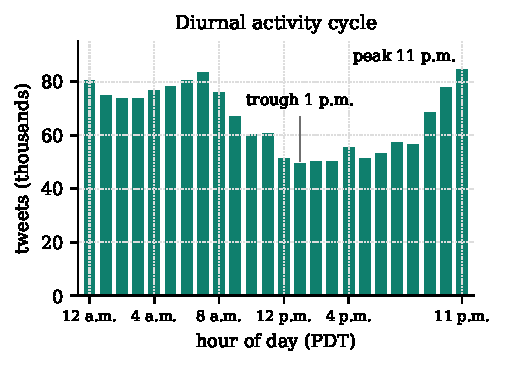
\includegraphics[width=\linewidth]{figures/fig2_diurnal.pdf}
  \caption{Diurnal activity cycle across the corpus (all 1.6M tweets).}
  \label{fig:diurnal}
\end{figure}

\textbf{Evaluating persona agents.} Park et al.\ \ecite{park2024} ground
agents in two-hour interviews with 1{,}052 people and score held-out
survey responses against each participant's own test--retest consistency;
Twin-2K-500 \ecite{twin2k} supplies a survey-based dataset with a repeat
wave for the same purpose. On social media, BluePrint \ecite{blueprint}
clusters anonymized Bluesky users into personas and poses next-action
prediction; BehaviorChain \ecite{behaviorchain}, TwinVoice, and
PersonaArena \ecite{personaarena} test persona simulation with
constructed or judge-scored scenarios. Wu et al.\ \ecite{boundary} review
this literature and find that fewer than half of validation studies
report behavioral variance, which is why we report the per-user
adherence distribution alongside the aggregate. Our benchmark differs
from all of these in scoring individual (not clustered) users on
real held-out behavior from a fully public corpus.

\textbf{Sentiment dynamics and contagion on Twitter.} Whether sentiment
spreads over ties has a long empirical record. Kramer et al.\
\ecite{kramer2014} established causal emotional contagion on Facebook
with very small effect sizes; Ferrara and Yang \ecite{ferrara2015}
measured about a 4\% over-exposure effect on Twitter with a
scarcely-susceptible majority; Charlton et al.\ \ecite{charlton2016}
found that sentiment levels of stable @-mention communities persist over
months, with shifts traceable to external events. Aral et al.\
\ecite{aral2009} and Shalizi and Thomas \ecite{shalizi2011} show that
observational contagion estimates are confounded with homophily, while
Tan et al.\ \ecite{tan2011} show that @-mention neighbors are nonetheless
a useful static prior for user-level sentiment. Our diffusion experiment
(\S\ref{sec:diffusion}) quantifies this trade-off predictively on a public
corpus: DeGroot averaging \ecite{degroot1974} over the real mention graph
versus each user's own history, with the Friedkin--Johnsen anchored
variant \ecite{friedkin1990} as the natural intermediate left to future
work.

\textbf{Relationship structure.} Kwak et al.\ \ecite{kwak2010}
established the large-scale structural view of Twitter; Huberman et al.\
\ecite{huberman2009} showed that the sparse network of reciprocal
@-interactions, not the follower graph, is the network that matters; Cha
et al.\ \ecite{cha2010} showed that mention-based attention concentrates
on celebrities independently of follower count. Horton and Wohl
\ecite{horton1956} introduced the parasocial-interaction construct we
operationalize on mention pairs.


\begin{figure}[htb]
  \centering
  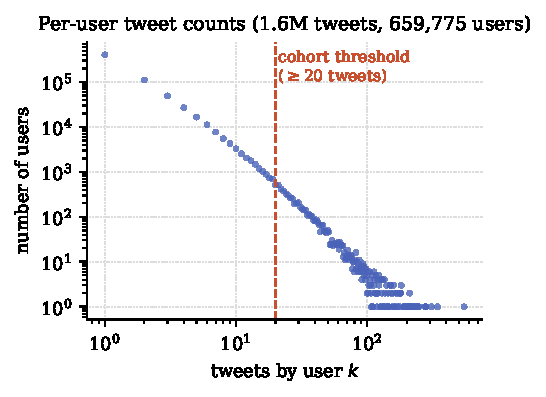
\includegraphics[width=\linewidth]{figures/fig1_user_distribution.pdf}
  \caption{Per-user tweet counts are heavy-tailed. The cohort threshold
  ($\geq 20$ tweets) admits 6{,}245 users covering 226{,}202 tweets.}
  \label{fig:dist}
\end{figure}

\textbf{Data.} Sentiment140 \ecite{sentiment140} provides 1.6M tweets
from April--June 2009, distantly labeled for sentiment by emoticons. It
remains one of the few large fully-public full-text tweet corpora: since
the 2023 restriction of the X API, tweet-ID ``hydration'' workflows that
most academic Twitter datasets rely on are effectively defunct, making
full-text corpora the practical substrate for new work. To our knowledge
it has been used almost exclusively for classifier benchmarking; we use
its per-user timelines and @-mention graph instead. TweetEval
\ecite{tweeteval} standardizes tweet classification benchmarks and
supplies pretrained classifiers usable as realism scorecards; Golder and
Macy \ecite{golder2011} document the diurnal mood cycle we recover in
Figure~\ref{fig:diurnal}.

\section{Dataset and Cohort}
\label{sec:dataset}




















\begin{figure}[t]
\centering
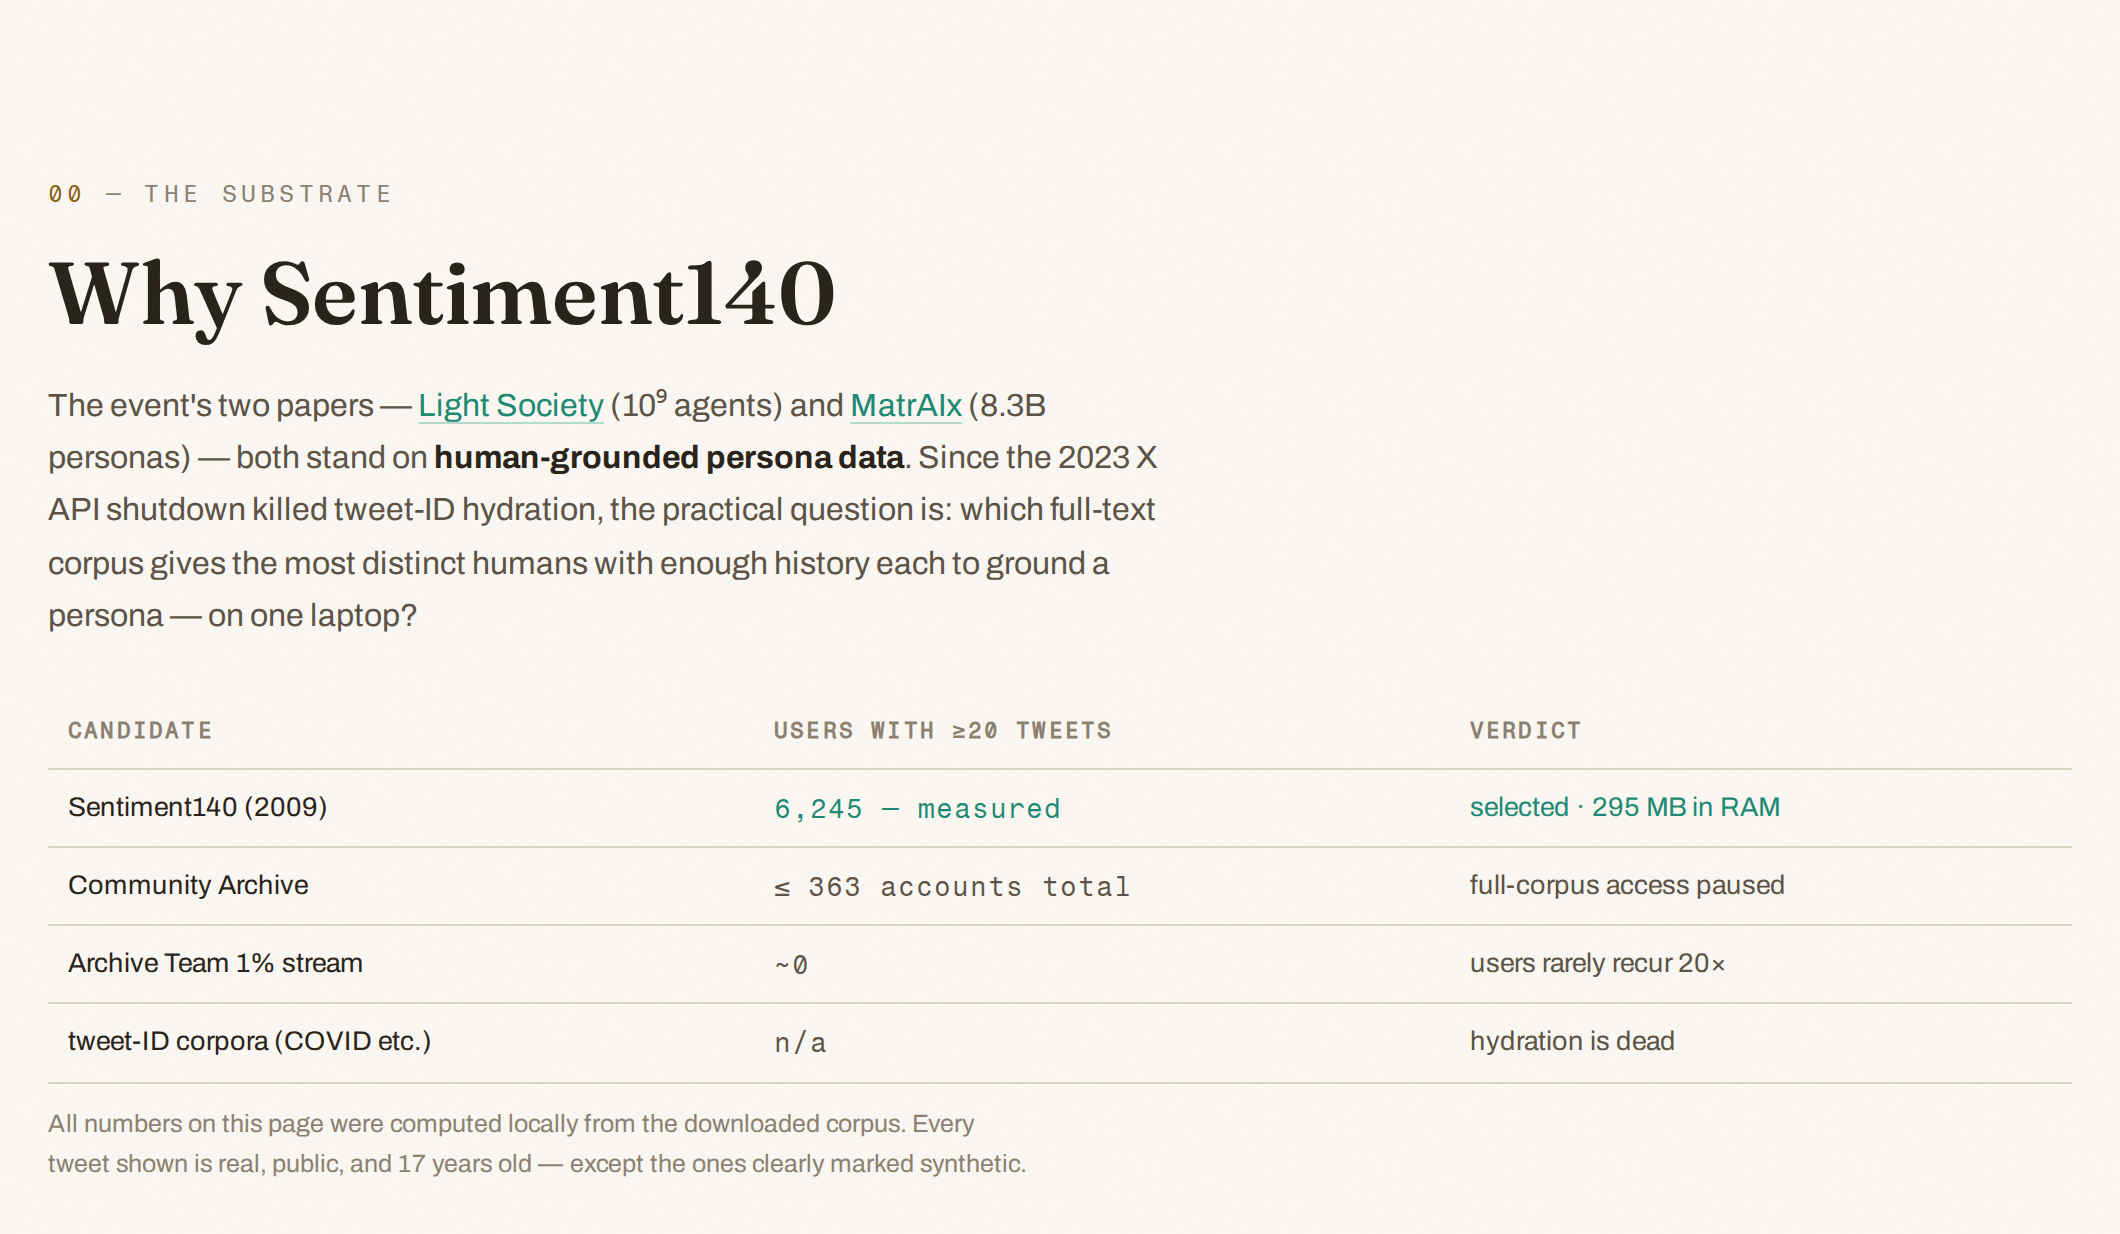
\includegraphics[width=\columnwidth]{figures/fig9_ui_data_light.png}
\caption{Dataset selection in the interactive explainer
(\url{https://popsim.micahstubbs.ai/\#data}): candidate corpora compared on
the number of distinct users with at least 20 tweets.}
\label{fig:ui-data}
\end{figure}

Sentiment140 loads from one CSV into 295\,MB of memory: 1{,}600{,}000 tweets,
659{,}775 distinct users, 48 days, balanced 800K/800K
negative/positive labels. Figure~\ref{fig:dist} shows the heavy-tailed per-user
activity distribution. We define the \textbf{persona cohort} as the 6{,}245
users with at least 20 tweets (226{,}202 tweets; mean 36.2, median 28 per
user; mean per-user activity span ${\sim}50$ days). The corpus retains a strong
diurnal rhythm (Figure~\ref{fig:diurnal}), with a peak at 11\,p.m.\ and a trough
at 1\,p.m.\ PDT, usable for calibrating agent posting schedules \ecite{golder2011}. Selection among candidate
corpora was itself empirical (Figure~\ref{fig:ui-data}): the Community Archive holds only 363 accounts;
the Archive Team 1\% stream rarely observes a user 20 times; ID-only corpora
cannot be hydrated. Sentiment140 maximizes the number of distinct humans with
enough history to ground a persona while fitting in RAM.


























\begin{figure*}[t]
  \centering
  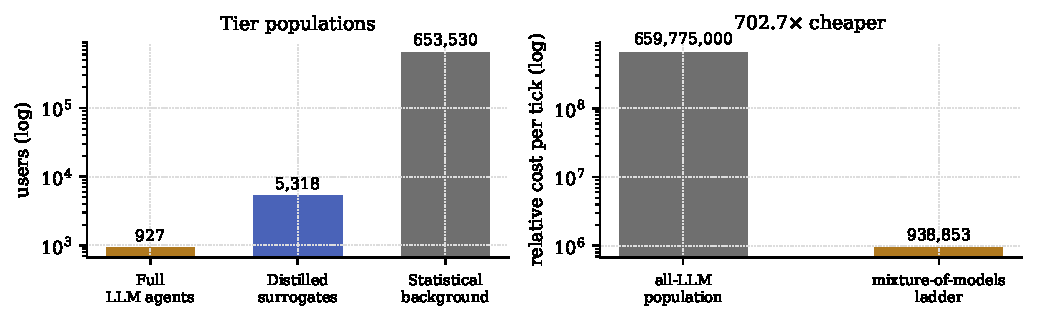
\includegraphics[width=.92\textwidth]{figures/fig4_ladder.pdf}
  \caption{The scale ladder. Left: tier populations (log scale). Right:
  relative cost of one simulation tick, all-LLM versus the ladder.}
  \label{fig:ladder}
\end{figure*}

\section{Persona Mining}
\label{sec:personas}

Following MatrAIx's human-grounded persona construction at hackathon scale,
each cohort user becomes a persona card computed from their real timeline:
sentiment disposition (share of positive tweets), verbosity (words/tweet),
mention rate, peak posting hour, activity span, and characteristic vocabulary.
Unlike survey-grounded profiles, these personas carry temporal behavior
(posting cadence, diurnal phase) directly usable to drive simulation ticks. The
cohort skews positive (59\% vs.\ the corpus's balanced 50\%), a selection
effect worth modeling rather than ignoring: highly active users differ from the
population they are drawn from.

\section{The Mixture-of-Models Scale Ladder}
\label{sec:ladder}


\begin{figure}[!b]
  \centering
  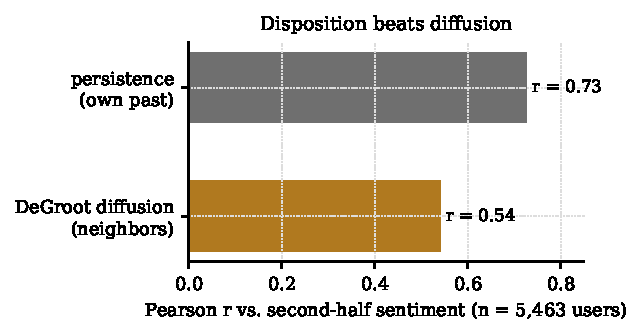
\includegraphics[width=\linewidth]{figures/fig3_diffusion.pdf}
  \caption{Predicting second-half sentiment from first-half state. Simple
  persistence outperforms DeGroot diffusion over the real mention graph.}
  \label{fig:diffusion}
\end{figure}

Heterogeneous agent cost is Light Society's central efficiency device
\ecite{lightsociety} and has since appeared as core/background splits
\ecite{hybriddiffusion}, structural grouping \ecite{toposim}, prototype
routing \ecite{aps}, and whole-agent surrogates \ecite{poorman}: full LLMs
only where fidelity demands them. We instantiate the same ladder sized to
one node (Figure~\ref{fig:ladder}): \textbf{full LLM agents} for the 927 users
with $\geq 50$ tweets (enough signal to condition a frontier model);
\textbf{distilled surrogates} (persona-conditioned small models) for the 5{,}318
users with 20--49 tweets; and a \textbf{statistical background} tier (rate and
sentiment samplers) for the remaining 653{,}530 users. Under a relative cost
model of $1000:1:0.01$ units per agent-tick, the ladder costs $9.39\times10^5$
units per tick versus $6.60\times10^8$ for an all-LLM population, a
$702.7\times$ reduction under the nominal cost model, with the full-LLM tier
reserved for the users who carry most of the observable signal. APS
\ecite{aps} reports a measured $381\times$ reduction at $10^7$ agents against
a full-LLM reference; we do not measure fidelity loss here.


















\begin{figure*}[t]
\centering
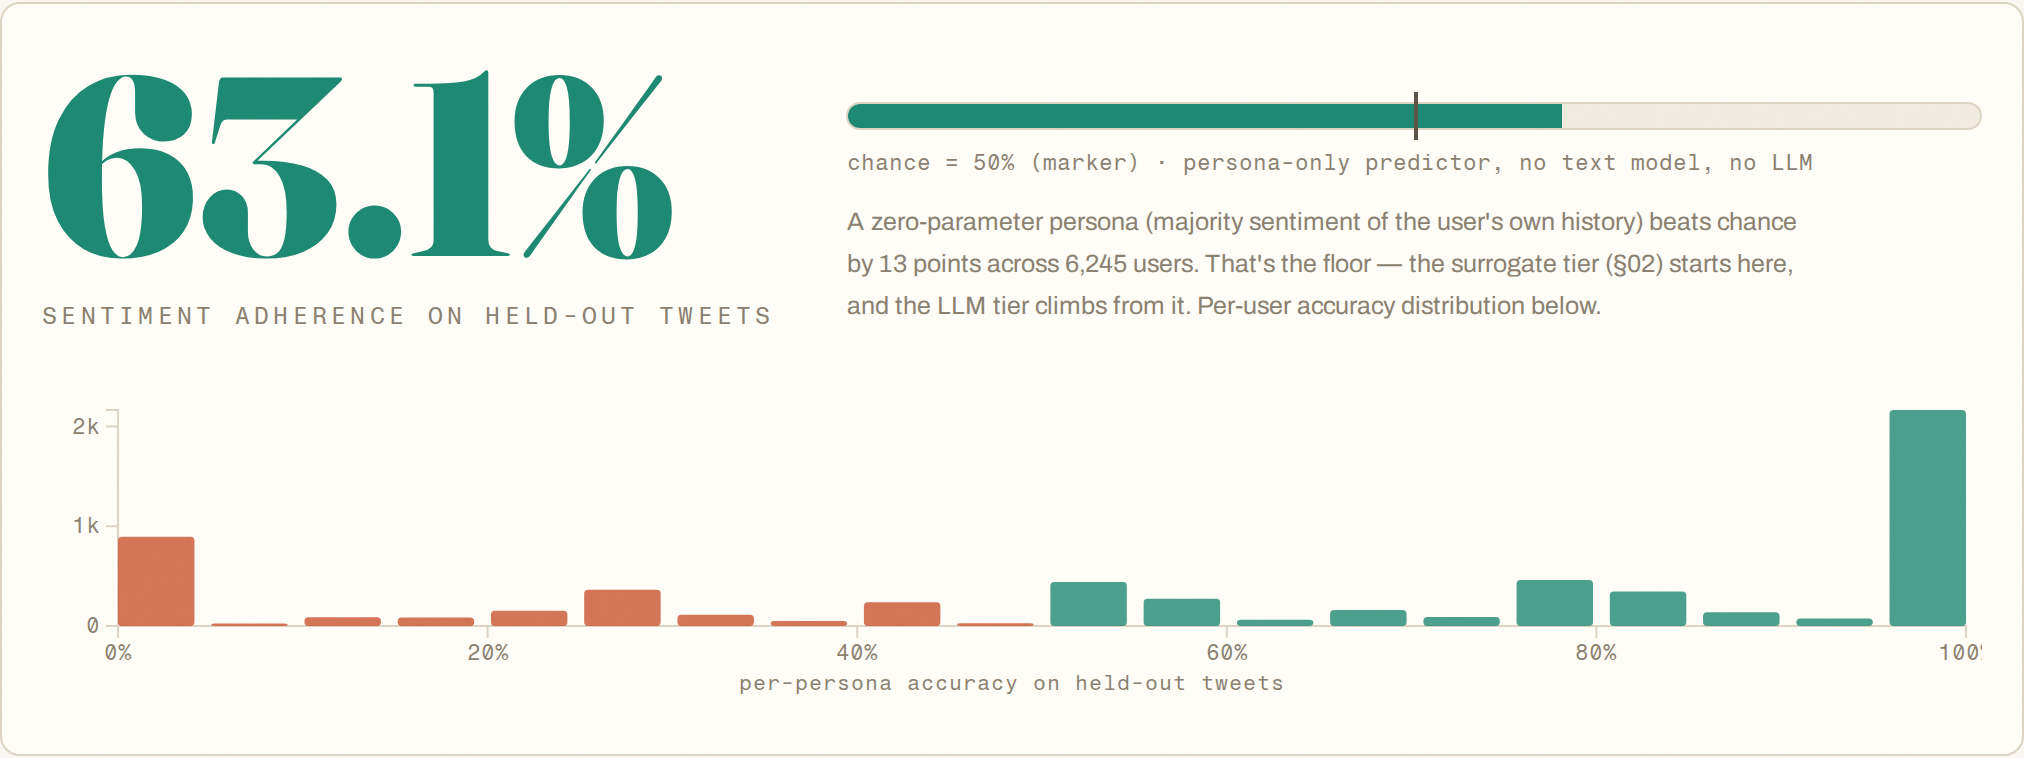
\includegraphics[width=.92\textwidth]{figures/fig8_ui_adherence_light.png}
\caption{The benchmark section of the interactive explainer
(\url{https://popsim.micahstubbs.ai/\#adherence}): the 63.1\% zero-parameter
baseline against the 50\% chance marker, and the per-persona accuracy
distribution over held-out tweets.}
\label{fig:ui-adherence}
\end{figure*}

\section{Does Sentiment Diffuse? A Validated Negative Result}
\label{sec:diffusion}


\begin{figure*}[t]
  \centering
  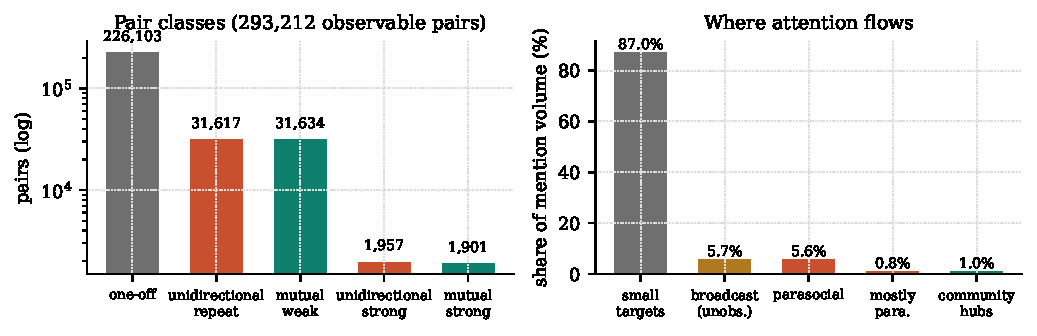
\includegraphics[width=.92\textwidth]{figures/fig6_parasocial.pdf}
  \caption{Left: relationship classes among the 293{,}212 pairs with
  observable reciprocity. Right: share of total mention volume by target
  class; parasocial + broadcast attention outweighs reciprocating community
  hubs by an order of magnitude.}
  \label{fig:parasocial}
\end{figure*}

The cohort contains a real directed interaction graph: 31{,}515 @-mention
events between cohort members. Light Society validates simulations with
opinion-diffusion experiments; we run the corresponding test \emph{against
ground truth}. Each user is seeded with their first-half sentiment; DeGroot
mixing \ecite{degroot1974}
($s_{t+1} = 0.7\,s_t + 0.3\,\bar{s}_{\mathcal{N}}$,
10 steps, edge weights = mention counts) evolves states over the real graph;
we then ask which predictor better recovers each user's \emph{second-half}
sentiment (users with $\geq 5$ tweets in each half; $n=5{,}463$).

Persistence wins (Figure~\ref{fig:diffusion}): $r=0.73$ for a user's own past
versus $r=0.54$ after diffusion; restricting to graph-connected users widens
the gap ($0.72$ vs.\ $0.40$). Neighbor-mixing strictly destroys predictive
information at this horizon. \textbf{Disposition beats diffusion}: over 48
days, who a person is outweighs who they talk to. This is the predictive face
of a well-known identification problem: in observational network data,
apparent contagion is largely homophily \ecite{aral2009}, and the two are
generically confounded \ecite{shalizi2011}. Our test does not show that
influence is absent, only that averaging over neighbors adds no information
beyond a user's own history at a 24-day horizon, in line with the ${\sim}4\%$
exposure effects Ferrara and Yang \ecite{ferrara2015} measure and the
month-scale stability Charlton et al.\ \ecite{charlton2016} observe on the
mention graph. For simulator design the
implication is direct: a population world model that over-weights social
contagion will be \emph{less} accurate than one grounded in stable personas,
which is why persona grounding (\S\ref{sec:personas}) matters. Static
neighbor information may still help as a prior \ecite{tan2011}; what fails is
dynamic mixing.





\section{Relationship Strength and Parasocial Structure}
\label{sec:parasocial}

To model whom agents should talk to, we quantify relationship structure over
the full mention graph (all 1.6M tweets). For unordered pairs where both users
author tweets in the sample (so silence is observed, not censored;
$n=293{,}212$ pairs), we score reciprocity $r=\min(w_{ab},w_{ba})/\max(w_{ab},w_{ba})$
and strength $\log(1{+}\text{total})\cdot\log(1{+}\text{days})\cdot(1{+}r)$,
and classify pairs by mutuality and volume (Figure~\ref{fig:parasocial},
left). Genuine relationships are rare: 77\% of pairs are one-off contacts,
echoing Huberman et al.'s finding that the network of reciprocal
@-interaction is far sparser than the declared graph \ecite{huberman2009}.
Sustained one-way attachments (\emph{unidirectional strong}:
$\geq 5$ mentions, zero returned; 1{,}957 pairs) are as numerous as strong
mutual bonds (1{,}901 pairs). For every observable friendship there is
roughly one unrequited attachment.

At the account level, among in-sample targets with $\geq 20$ distinct
mentioners, 408 reciprocate under 5\% of their audience, operationally
\emph{parasocial}
\ecite{horton1956},
including 2009-era celebrities
(\texttt{wossy}, \texttt{ashleytisdale}, \texttt{tomfelton}) who tweet but do
not talk back (the mention concentration on celebrities that Cha et al.\
\ecite{cha2010} documented), while 163 \emph{community hubs} of comparable audience
reciprocate 30--53\%. A further 524 broadcast targets (e.g.\
\texttt{jonasbrothers}: 1{,}901 distinct fans in 48 days) never author a
sampled tweet, so their reciprocity is unobservable and we label rather than
classify them. By volume, 12.1\% of all mention traffic flows to
broadcast/parasocial accounts versus 1.0\% to reciprocating hubs
(Figure~\ref{fig:parasocial}, right).

The architectural implication joins \S\ref{sec:ladder}: simulated populations
need a \textbf{broadcast tier}, and it is nearly free, since parasocial
edges are one-directional by construction. The celebrity side requires no
agent at all, only a content feed.









\section{A Behavioral-Adherence Benchmark on Sentiment140}
\label{sec:benchmark}

















MatrAIx's headline metric, whether persona agents behave like their personas,
currently lacks a public, fixed-protocol instantiation on real held-out
behavior of individual users: Park et al.\ \ecite{park2024} and Twin-2K-500
\ecite{twin2k} score held-out survey items, and BluePrint \ecite{blueprint}
scores next actions for anonymized persona clusters rather than individuals.
We contribute one on an existing fully-public corpus, with live results in the
interactive explainer (Figure~\ref{fig:ui-adherence}).

\textbf{Protocol (fixed).} Cohort: the 6{,}245 Sentiment140 users with
$\geq 20$ tweets. Per user, order tweets by time; train = first 80\%, test =
last 20\% (minimum 4). Metric: fraction of the 42{,}998 held-out tweets whose
sentiment label the persona model predicts, reported overall and as the
per-user distribution. Rules: no access to any user's test tweets at training
or persona-construction time; train-tweet text is unrestricted (features,
pretrained classifiers, persona-conditioned LLM prompting, fine-tuning).






\begin{figure}[H]
  \centering
  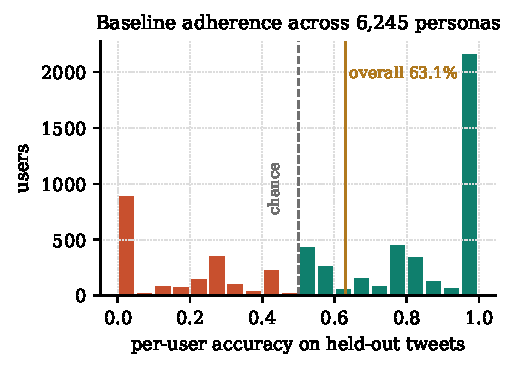
\includegraphics[width=\linewidth]{figures/fig5_adherence.pdf}
  \caption{Per-user adherence of the zero-parameter persona baseline on
  held-out tweets. Overall: 63.1\% over 42{,}998 tweets.}
  \label{fig:adherence}
\end{figure}

\textbf{Baseline.} The zero-parameter persona, which predicts each user's
train-majority sentiment, attains \textbf{63.1\%} (chance: 50\%,
label-balanced corpus). Figure~\ref{fig:adherence} shows the per-user
distribution: bimodal, with a large mass of highly consistent users and a
long tail of volatile ones for whom persona-only prediction fails. This is the
floor a surrogate tier starts from and an LLM tier must climb. Reporting the
distribution, not only the mean, follows Wu et al.'s \ecite{boundary}
recommendation that simulation evaluations report behavioral variance.

\textbf{The bar.} MatrAIx reports 91.5\% behavioral adherence across ten
attributes in four environments. The protocols are not comparable: theirs
measures declared-attribute expression in synthetic interactions, while ours
measures real held-out behavior. We therefore frame 91.5\% as an aspirational
bar on our protocol, not a record to break on equal terms. The benchmark poses an
open question: how far above 63.1\% can persona-conditioned models go on
real, noisy, distantly-labeled human behavior?





\section{Limitations}

Our substrate is 2009 Twitter: 140-character posts, no quote tweets, no
algorithmic feed; behavioral constants observed here need not transfer to
modern platforms. Sentiment labels are distant (emoticon-derived) and noisy.
The corpus is a partial sample, which censors reciprocity; we mitigate by
restricting reciprocity claims to in-sample authors with audience $\geq 20$
and labeling out-of-sample targets as unobserved. The scale-ladder cost model
uses nominal relative unit costs, not measured wall-clock inference costs. The
diffusion experiment tests one model (DeGroot, $\alpha=0.7$, 10 steps) at one
horizon; richer contagion models, most naturally Friedkin--Johnsen
\ecite{friedkin1990}, which anchors each agent to its initial state and
interpolates between persistence and DeGroot, could yet beat persistence; and
because homophily and influence are not separable in observational data
\ecite{shalizi2011}, our result concerns prediction, not causation. Finally, the
adherence benchmark measures a single behavioral dimension (sentiment);
MatrAIx-style multi-attribute adherence on this cohort is natural future work.

\section{Conclusion}

The methodology of billion-agent social simulators is not confined to
billion-agent budgets, a point made independently by Itkin \ecite{poorman}
for LLM-cloned surrogates; our contribution is to do it with real people, a
real graph, and real held-out behavior. On one machine and one public dataset we reproduced the
persona-grounding and mixture-of-models patterns of Light Society and MatrAIx,
validated a diffusion assumption against ground truth (and found it wanting),
mapped the parasocial structure a realistic simulator must include, and left
behind a fixed, public behavioral-adherence benchmark with a 63.1\% baseline
and a 91.5\% bar. The gap between those numbers is, we hope, an invitation.

\subsection*{Artifact Availability}
The interactive explainer shown in Figures~\ref{fig:ui-data}
and~\ref{fig:ui-adherence} is live at \url{https://popsim.micahstubbs.ai}.
All analysis code, data pipelines, the benchmark protocol, and the source of
this paper are at \url{https://github.com/micahstubbs/pop-world-model-sim};
the deployed site source is at \url{https://github.com/micahstubbs/popsim}.

\subsection*{Acknowledgments}
Built at the Postlabor.dev ``Building Economic World Models'' Simulation Build
Night (August 2026, \url{https://luma.com/th01qwp1}). We thank Jake Schwartz
for collaboration during the build
night, and the event hosts
Clovis Vinant-Tang (\url{https://x.com/ClovisVinant}),
Tanzeela Khan (\url{https://x.com/tanzealous}), and
Yvonne Chen (\url{https://x.com/ycyvonne_})
for organizing the evening that made this work possible.



\begin{thebibliography}{99}\small

\bibitem{lightsociety}
H.~Guan, J.~He, L.~Fan, Z.~Ren, S.~He, X.~Yu, Y.~Chen, X.~Xu, S.~Zheng,
Y.~Gao, E.~Chen, T.-Y.~Liu, Z.~Liu.
\newblock \reftitle{lightsociety}{Modeling Earth-Scale
Human-Like Societies with One Billion Agents}.
\newblock \emph{arXiv:2506.12078}, 2025.

\bibitem{matraix}
X.~Li, Y.~Hao, J.~Hou, J.~Huang, et al.
\newblock \reftitle{matraix}{MatrAIx: Simulating the
World with 8.3 Billion Persona Agents}.
\newblock \emph{arXiv:2608.04205}, 2026.

\bibitem{park2023}
J.~S. Park, J.~O'Brien, C.~J. Cai, M.~R. Morris, P.~Liang, M.~S. Bernstein.
\newblock \reftitle{park2023}{Generative Agents:
Interactive Simulacra of Human Behavior}.
\newblock In \emph{Proc.\ UIST}, 2023. arXiv:2304.03442.

\bibitem{sentiment140}
A.~Go, R.~Bhayani, L.~Huang.
\newblock \reftitle{sentiment140}{Twitter
Sentiment Classification using Distant Supervision}.
\newblock Stanford CS224N Project Report, 2009.

\bibitem{tweeteval}
F.~Barbieri, J.~Camacho-Collados, L.~Espinosa-Anke, L.~Neves.
\newblock \reftitle{tweeteval}{TweetEval:
Unified Benchmark and Comparative Evaluation for Tweet Classification}.
\newblock In \emph{Findings of EMNLP}, 2020. arXiv:2010.12421.

\bibitem{kwak2010}
H.~Kwak, C.~Lee, H.~Park, S.~Moon.
\newblock \reftitle{kwak2010}{What
is Twitter, a Social Network or a News Media?}
\newblock In \emph{Proc.\ WWW}, 2010.

\bibitem{horton1956}
D.~Horton, R.~R. Wohl.
\newblock \reftitle{horton1956}{Mass
Communication and Para-Social Interaction: Observations on Intimacy at a
Distance}.
\newblock \emph{Psychiatry}, 19(3):215--229, 1956.

\bibitem{degroot1974}
M.~H. DeGroot.
\newblock \reftitle{degroot1974}{Reaching a
Consensus}.
\newblock \emph{Journal of the American Statistical Association},
69(345):118--121, 1974.

\bibitem{oasis}
Z.~Yang, Z.~Zhang, Z.~Zheng, Y.~Jiang, Z.~Gan, Z.~Wang, Z.~Ling, J.~Chen,
M.~Ma, B.~Dong, P.~Gupta, S.~Hu, Z.~Yin, G.~Li, X.~Jia, L.~Wang, B.~Ghanem,
H.~Lu, C.~Lu, W.~Ouyang, Y.~Qiao, P.~Torr, J.~Shao.
\newblock \reftitle{oasis}{OASIS: Open Agent Social Interaction Simulations
with One Million Agents}.
\newblock In \emph{Proc.\ ICML}, 2025. arXiv:2411.11581.

\bibitem{agentsociety}
J.~Piao, Y.~Yan, J.~Zhang, N.~Li, J.~Yan, X.~Lan, Z.~Lu, Z.~Zheng, J.~Y. Wang,
D.~Zhou, C.~Gao, F.~Xu, F.~Zhang, K.~Rong, J.~Su, Y.~Li.
\newblock \reftitle{agentsociety}{AgentSociety: Large-Scale Simulation of
LLM-Driven Generative Agents Advances Understanding of Human Behaviors and
Society}.
\newblock \emph{arXiv:2502.08691}, 2025.

\bibitem{ysocial}
G.~Rossetti, M.~Stella, R.~Cazabet, K.~Abramski, E.~Cau, S.~Citraro,
A.~Failla, R.~Improta, V.~Morini, V.~Pansanella.
\newblock \reftitle{ysocial}{Y Social: an LLM-powered Social Media Digital
Twin}.
\newblock \emph{arXiv:2408.00818}, 2024.

\bibitem{socioverse}
X.~Zhang, J.~Lin, X.~Mou, S.~Yang, X.~Liu, L.~Sun, H.~Lyu, Y.~Yang, W.~Qi,
Y.~Chen, G.~Li, L.~Yan, Y.~Hu, S.~Chen, Y.~Wang, X.~Huang, J.~Luo, S.~Tang,
L.~Wu, B.~Zhou, Z.~Wei.
\newblock \reftitle{socioverse}{SocioVerse: A World Model for Social
Simulation Powered by LLM Agents and A Pool of 10 Million Real-World Users}.
\newblock \emph{arXiv:2504.10157}, 2025.

\bibitem{aps}
Q.~Zheng, Y.~Gao, S.~He, H.~Guan, Y.~Tian, J.~Feng, M.~Wang, S.~Zheng,
Z.~Liu.
\newblock \reftitle{aps}{APS: Bias-Controlled Adaptive Prototype Simulation
for Population-Scale LLM Agents}.
\newblock \emph{arXiv:2605.27419}, 2026.

\bibitem{poorman}
I.~Itkin.
\newblock \reftitle{poorman}{Poor Man's Agentic Modeling: Simulating Large
LLM-Agent Societies on a Laptop}.
\newblock \emph{arXiv:2608.11215}, 2026.

\bibitem{hybriddiffusion}
X.~Li, Z.~Guo, Q.~Guo, H.~Jin, W.~Ma, M.~Zhang.
\newblock \reftitle{hybriddiffusion}{Integrating LLM and Diffusion-Based
Agents for Social Simulation}.
\newblock \emph{arXiv:2510.16366}, 2025.

\bibitem{toposim}
Y.~Xu, S.~Zhang, Y.~Zhou, S.~Zeng, L.~V.~S. Lakshmanan, C.~Ma.
\newblock \reftitle{toposim}{Topology-Aware LLM-Driven Social Simulation: A
Unified Framework for Efficient and Realistic Agent Dynamics}.
\newblock \emph{arXiv:2604.18011}, 2026.

\bibitem{scaling}
C.~Ziems, W.~Held, S.~D. Karaca, D.~Grusky, T.~Hashimoto, D.~Yang.
\newblock \reftitle{scaling}{Will Scaling Improve Social Simulation with
LLMs?}
\newblock \emph{arXiv:2607.02464}, 2026.

\bibitem{park2024}
J.~S. Park, C.~Q. Zou, J.~Kamphorst, N.~Egan, A.~Shaw, B.~M. Hill, C.~Cai,
M.~R. Morris, P.~Liang, R.~Willer, M.~S. Bernstein.
\newblock \reftitle{park2024}{LLM Agents Grounded in Self-Reports Enable
General-Purpose Simulation of Individuals}.
\newblock \emph{arXiv:2411.10109}, 2024.

\bibitem{twin2k}
O.~Toubia, G.~Z. Gui, T.~Peng, D.~J. Merlau, A.~Li, H.~Chen.
\newblock \reftitle{twin2k}{Twin-2K-500: A Dataset for Building Digital Twins
of over 2,000 People Based on Their Answers to over 500 Questions}.
\newblock \emph{Marketing Science}, 2025. arXiv:2505.17479.

\bibitem{blueprint}
A.~B\"uck-Kaeffer, J.~Q. Chooi, D.~Zhao, M.~Puelma Touzel, K.~Pelrine,
J.-F. Godbout, R.~Rabbany, Z.~Yang.
\newblock \reftitle{blueprint}{BluePrint: A Social Media User Dataset for
LLM Persona Evaluation and Training}.
\newblock \emph{arXiv:2510.02343}, 2025.

\bibitem{behaviorchain}
R.~Li, H.~Xia, X.~Yuan, Q.~Dong, L.~Sha, W.~Li, Z.~Sui.
\newblock \reftitle{behaviorchain}{How Far are LLMs from Being Our Digital
Twins? A Benchmark for Persona-Based Behavior Chain Simulation}.
\newblock In \emph{Findings of ACL}, 2025. arXiv:2502.14642.

\bibitem{personaarena}
W.~Shi, J.~Lian, M.~Wu, H.~Qin, M.~Zhou, X.~Xie, N.~Chao, H.~Liao.
\newblock \reftitle{personaarena}{PersonaArena: Dynamic Simulation for
Evaluating and Enhancing Persona-Level Role-Playing in Large Language
Models}.
\newblock In \emph{Findings of ACL}, 2026. arXiv:2605.17044.

\bibitem{boundary}
Z.~Wu, R.~Peng, T.~Ito, M.~Onizuka, C.~Xiao.
\newblock \reftitle{boundary}{LLM-Based Social Simulations Require a
Boundary}.
\newblock In \emph{Proc.\ ICML (Position Papers)}, 2026. arXiv:2506.19806.

\bibitem{kramer2014}
A.~D.~I. Kramer, J.~E. Guillory, J.~T. Hancock.
\newblock \reftitle{kramer2014}{Experimental Evidence of Massive-Scale
Emotional Contagion through Social Networks}.
\newblock \emph{PNAS}, 111(24):8788--8790, 2014.

\bibitem{ferrara2015}
E.~Ferrara, Z.~Yang.
\newblock \reftitle{ferrara2015}{Measuring Emotional Contagion in Social
Media}.
\newblock \emph{PLoS ONE}, 10(11):e0142390, 2015.

\bibitem{charlton2016}
N.~Charlton, C.~Singleton, D.~V. Greetham.
\newblock \reftitle{charlton2016}{In the Mood: The Dynamics of Collective
Sentiments on Twitter}.
\newblock \emph{Royal Society Open Science}, 3(6):160162, 2016.

\bibitem{aral2009}
S.~Aral, L.~Muchnik, A.~Sundararajan.
\newblock \reftitle{aral2009}{Distinguishing Influence-Based Contagion from
Homophily-Driven Diffusion in Dynamic Networks}.
\newblock \emph{PNAS}, 106(51):21544--21549, 2009.

\bibitem{shalizi2011}
C.~R. Shalizi, A.~C. Thomas.
\newblock \reftitle{shalizi2011}{Homophily and Contagion Are Generically
Confounded in Observational Social Network Studies}.
\newblock \emph{Sociological Methods \& Research}, 40(2):211--239, 2011.

\bibitem{tan2011}
C.~Tan, L.~Lee, J.~Tang, L.~Jiang, M.~Zhou, P.~Li.
\newblock \reftitle{tan2011}{User-Level Sentiment Analysis Incorporating
Social Networks}.
\newblock In \emph{Proc.\ KDD}, 2011.

\bibitem{friedkin1990}
N.~E. Friedkin, E.~C. Johnsen.
\newblock \reftitle{friedkin1990}{Social Influence and Opinions}.
\newblock \emph{Journal of Mathematical Sociology}, 15(3--4):193--205, 1990.

\bibitem{huberman2009}
B.~A. Huberman, D.~M. Romero, F.~Wu.
\newblock \reftitle{huberman2009}{Social Networks that Matter: Twitter under
the Microscope}.
\newblock \emph{First Monday}, 14(1), 2009.

\bibitem{cha2010}
M.~Cha, H.~Haddadi, F.~Benevenuto, K.~P. Gummadi.
\newblock \reftitle{cha2010}{Measuring User Influence in Twitter: The
Million Follower Fallacy}.
\newblock In \emph{Proc.\ ICWSM}, 2010.

\bibitem{golder2011}
S.~A. Golder, M.~W. Macy.
\newblock \reftitle{golder2011}{Diurnal and Seasonal Mood Vary with Work,
Sleep, and Daylength across Diverse Cultures}.
\newblock \emph{Science}, 333(6051):1878--1881, 2011.

\end{thebibliography}

\end{document}
